\documentclass[sigconf,nonacm]{acmart}

\settopmatter{printacmref=false}
\setcopyright{none}
\renewcommand\footnotetextcopyrightpermission[1]{}
\pagestyle{plain}

\usepackage{graphicx}
\usepackage{booktabs}
\usepackage{array}

\title{Timebox: A Multi-Agent Calendar Planner for Student Workloads}

\author{Daniel Bernardes, 116246}
\affiliation{%
  \institution{Instituto Superior T\'ecnico}
  \city{Lisbon}
  \country{Portugal}}

\author{Pedro Silva, 116117}
\affiliation{%
  \institution{Instituto Superior T\'ecnico}
  \city{Lisbon}
  \country{Portugal}}

\renewcommand{\shortauthors}{Bernardes and Silva}

\begin{document}

\noindent
\includegraphics[width=1.8cm]{images/ist_logo_placeholder.png}\par\vspace{0.4em}

\begin{abstract}
Timebox is a desktop planning system that turns a student's natural-language workload description into a calendar through multi-agent critique and revision. An interpreter extracts tasks, deadlines, availability, and fixed commitments; five specialist agents inspect the planning state from different perspectives; and a planner-arbiter iteratively revises candidate calendars until a quorum accepts one or a fallback condition is reached. We evaluated the system on eight fixed student scenarios using deterministic mistake labels, a fixed qualitative judge, and cost tracing. The strongest result is not only a leaderboard: the same evaluation labels exposed repeated deadline failures, guided a Deadline Agent prompt revision, and reduced critical work-after-deadline mistakes from five to one in comparable Gemini runs.
\end{abstract}

\maketitle

\section{Problem}
Student planning is a multi-objective problem. A useful schedule must respect deadlines, distribute effort realistically, consider grade importance, leave room for uncertainty, and avoid harmful work patterns. These goals conflict: a deadline-safe plan can overload a low-energy student, while a relaxed plan can miss an academic commitment. We built Timebox to make these trade-offs explicit instead of hiding them inside one planner response.

The input is a free-form student request. The output is a week-style calendar with reasoning, critiques, validation labels, and JSON/ICS export. The system is implemented as an Electron and React desktop application backed by OpenRouter models.

\section{System Design}
Figure~\ref{fig:architecture} shows the final pipeline. The Interpreter Agent first converts natural language into structured planning data: current date, planning window, inferred availability, fixed commitments, student state, and task records with inferred deadlines. Specialist agents then produce independent task views:

\begin{itemize}
  \item Deadline Agent checks urgency and deadline ordering.
  \item Grade Agent prioritizes grade-relevant work.
  \item Effort Agent estimates workload and hidden effort.
  \item Wellbeing Agent watches overload and late-night work.
  \item Risk Agent identifies uncertainty and fragile plans.
\end{itemize}

The Planner-Arbiter creates a calendar proposal. The specialist agents critique it, and approval requires the configured quorum. If the system reaches the maximum number of revisions, it selects the best available calendar by critique severity and approvals. Validation is diagnostic rather than a hard gate: it records objective errors such as work after a deadline, invalid block times, explicit rest blocks, or unknown task IDs, but does not directly replace the agent acceptance mechanism.

\begin{figure}[t]
  \centering
  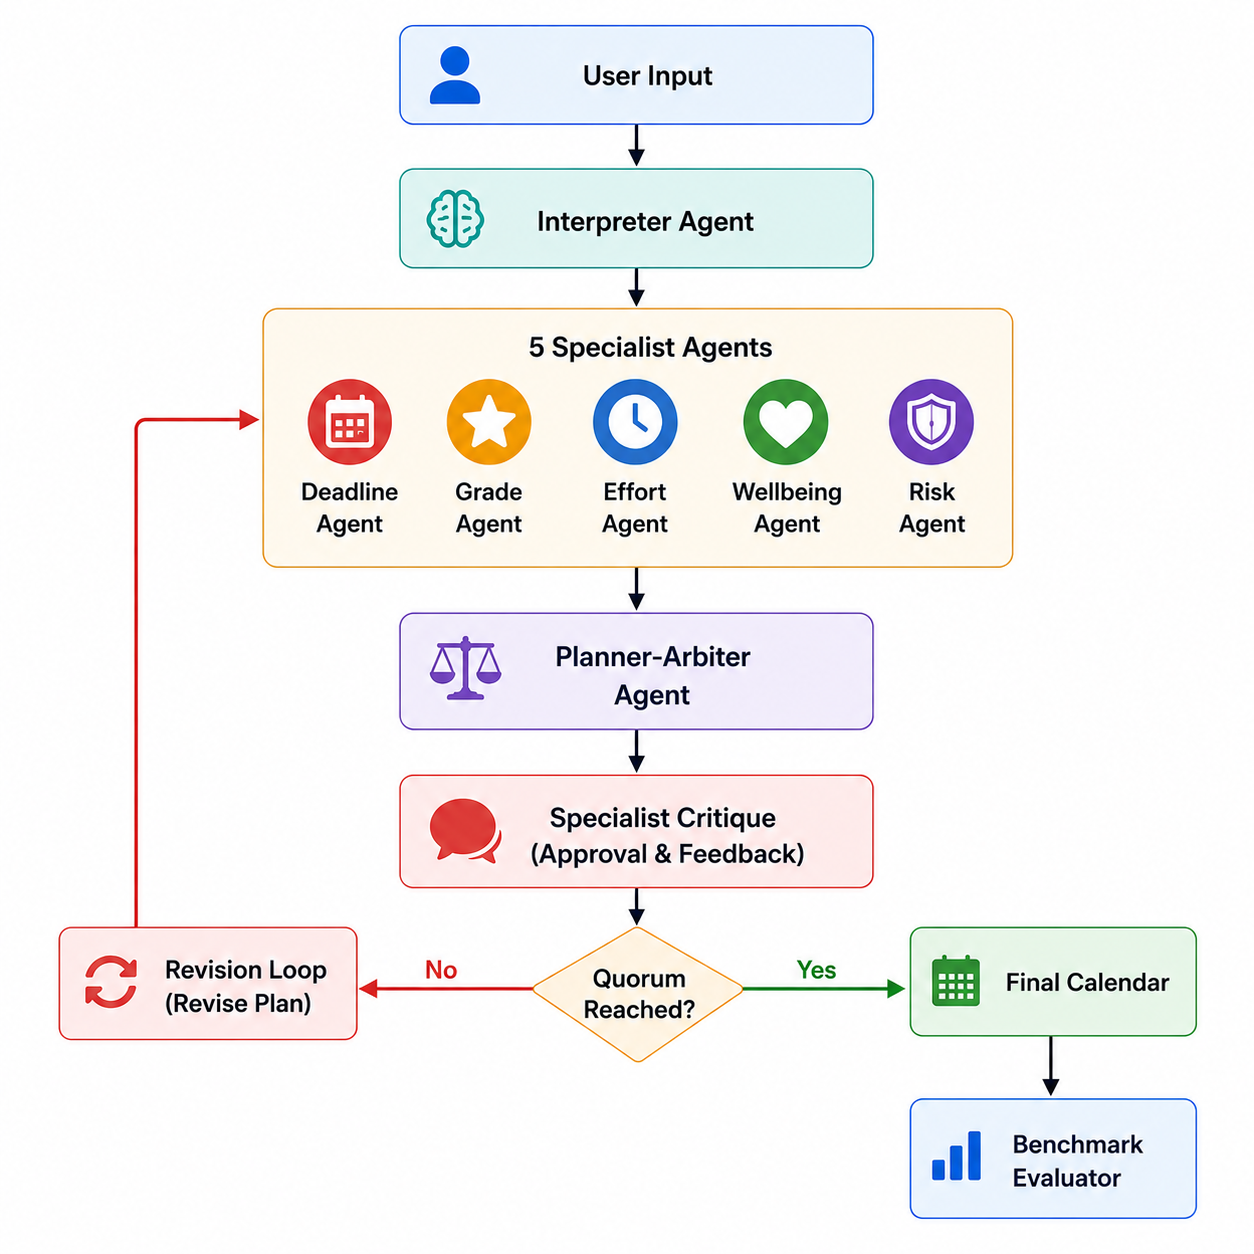
\includegraphics[width=\linewidth]{images/arquitecture.png}
  \caption{Timebox pipeline: interpretation, specialist task views, planner-arbiter generation, critique, revision, and calendar export.}
  \label{fig:architecture}
\end{figure}

\section{Evaluation Method}
We used eight fixed benchmark scenarios covering urgent deadlines, low energy, grade-weighted priorities, group coordination, fixed commitments, uncertain scope, exam revision, and part-time work. Each model used quorum five and up to three planner revisions. We recorded cost, token use, iterations, final critiques, deterministic mistakes, and a qualitative judge score.

The main comparison score in the analytics table is an adjusted value:

\[
\begin{split}
V = &\,0.70D + 0.15J + 0.15R\\
    &- 4C - 0.7M - P_{cost}
\end{split}
\]

Here \(D\) is deterministic schedule score, \(J\) is the fixed judge score scaled to 0--100, \(R\) is run reliability, \(C\) is critical mistakes per run, \(M\) is non-critical mistakes per run, and \(P_{cost}\) is a logarithmic cost penalty capped at 12 points. This keeps objective schedule quality dominant while still penalizing failures, critical labels, and operational cost.

The deterministic score is rule-based and does not call another model. It is computed from expected task coverage, deadline discipline, availability discipline, fixed-commitment handling, wellbeing, and revision efficiency. It uses the interpreter's structured output for task IDs and inferred deadlines; for example, validation emits \texttt{block\_after\_deadline} when a work block's end timestamp is later than that task's inferred deadline. This makes the score explainable, but also means it depends on the interpreter correctly extracting deadlines from natural language.

\section{Results}
Figure~\ref{fig:model-summary} and Table~\ref{tab:results} summarize the completed model comparison. Gemini 2.5 Flash Lite had the best adjusted value, despite Gemini 3.1 Flash Lite having slightly higher raw deterministic and judge scores, because Gemini 2.5 was cheaper and had fewer critical mistakes. DeepSeek V3.2 was substantially weaker in this orchestration setting: it accumulated more critical mistakes, used more iterations, and often failed to reach quorum.

\begin{figure}[t]
  \centering
  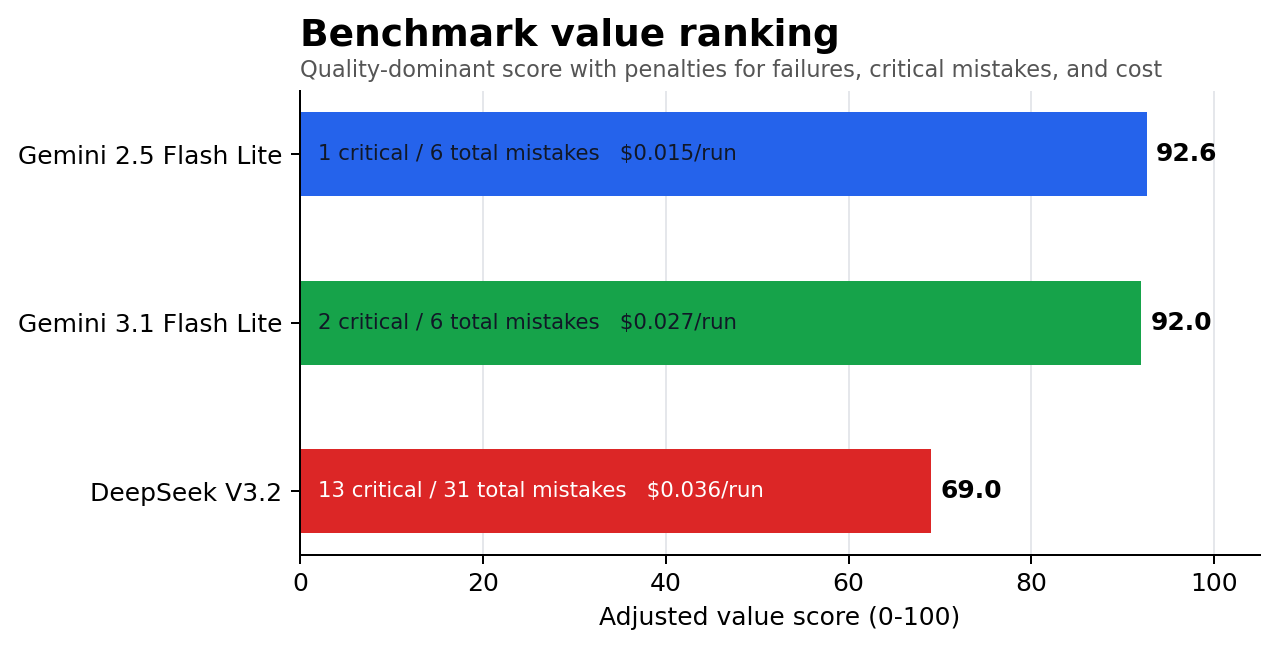
\includegraphics[width=\linewidth]{images/report_model_summary.png}
  \caption{Adjusted value ranking over the final eight-scenario benchmark. The chart shows the main comparison metric and annotates the operational reasons behind it.}
  \label{fig:model-summary}
\end{figure}

\begin{table}[t]
  \centering
  \caption{Aggregate results over eight scenarios. Cost is average USD per full planning run.}
  \label{tab:results}
  \begin{tabular}{lrrrr}
    \toprule
    Model & Adj. & Det. & Crit. & Cost \\
    \midrule
    Gemini 2.5 Flash Lite & 92.6 & 97.3 & 1 & \$0.015 \\
    Gemini 3.1 Flash Lite & 92.0 & 97.5 & 2 & \$0.027 \\
    DeepSeek V3.2 & 69.0 & 81.6 & 13 & \$0.036 \\
    \bottomrule
  \end{tabular}
\end{table}

We also attempted MiniMax M2.7, but it did not finish the benchmark in a usable time because OpenRouter responses were too slow and timeout-prone. We therefore treated it as DNF rather than mixing incomplete runs into the comparison.

\section{Prompt Improvement Case Study}
The most useful part of the benchmark was not the final ranking; it was the deterministic mistake labels. The first benchmark showed that deadline handling was the main critical failure mode. In particular, the system sometimes scheduled task work after the exact deadline timestamp.

We revised the Deadline Agent prompt to audit exact deadline timestamps and identify offending work blocks. Figure~\ref{fig:mistakes} compares the top mistake labels before and after the prompt change for the two Gemini models rerun under both prompts. Critical work-after-deadline mistakes dropped from five to one, and availability overruns dropped from eight to three. The remaining mistakes are more distributed, which is a better debugging state: no single critical failure dominates.

\begin{figure*}[t]
  \centering
  \begin{minipage}{0.49\textwidth}
    \centering
    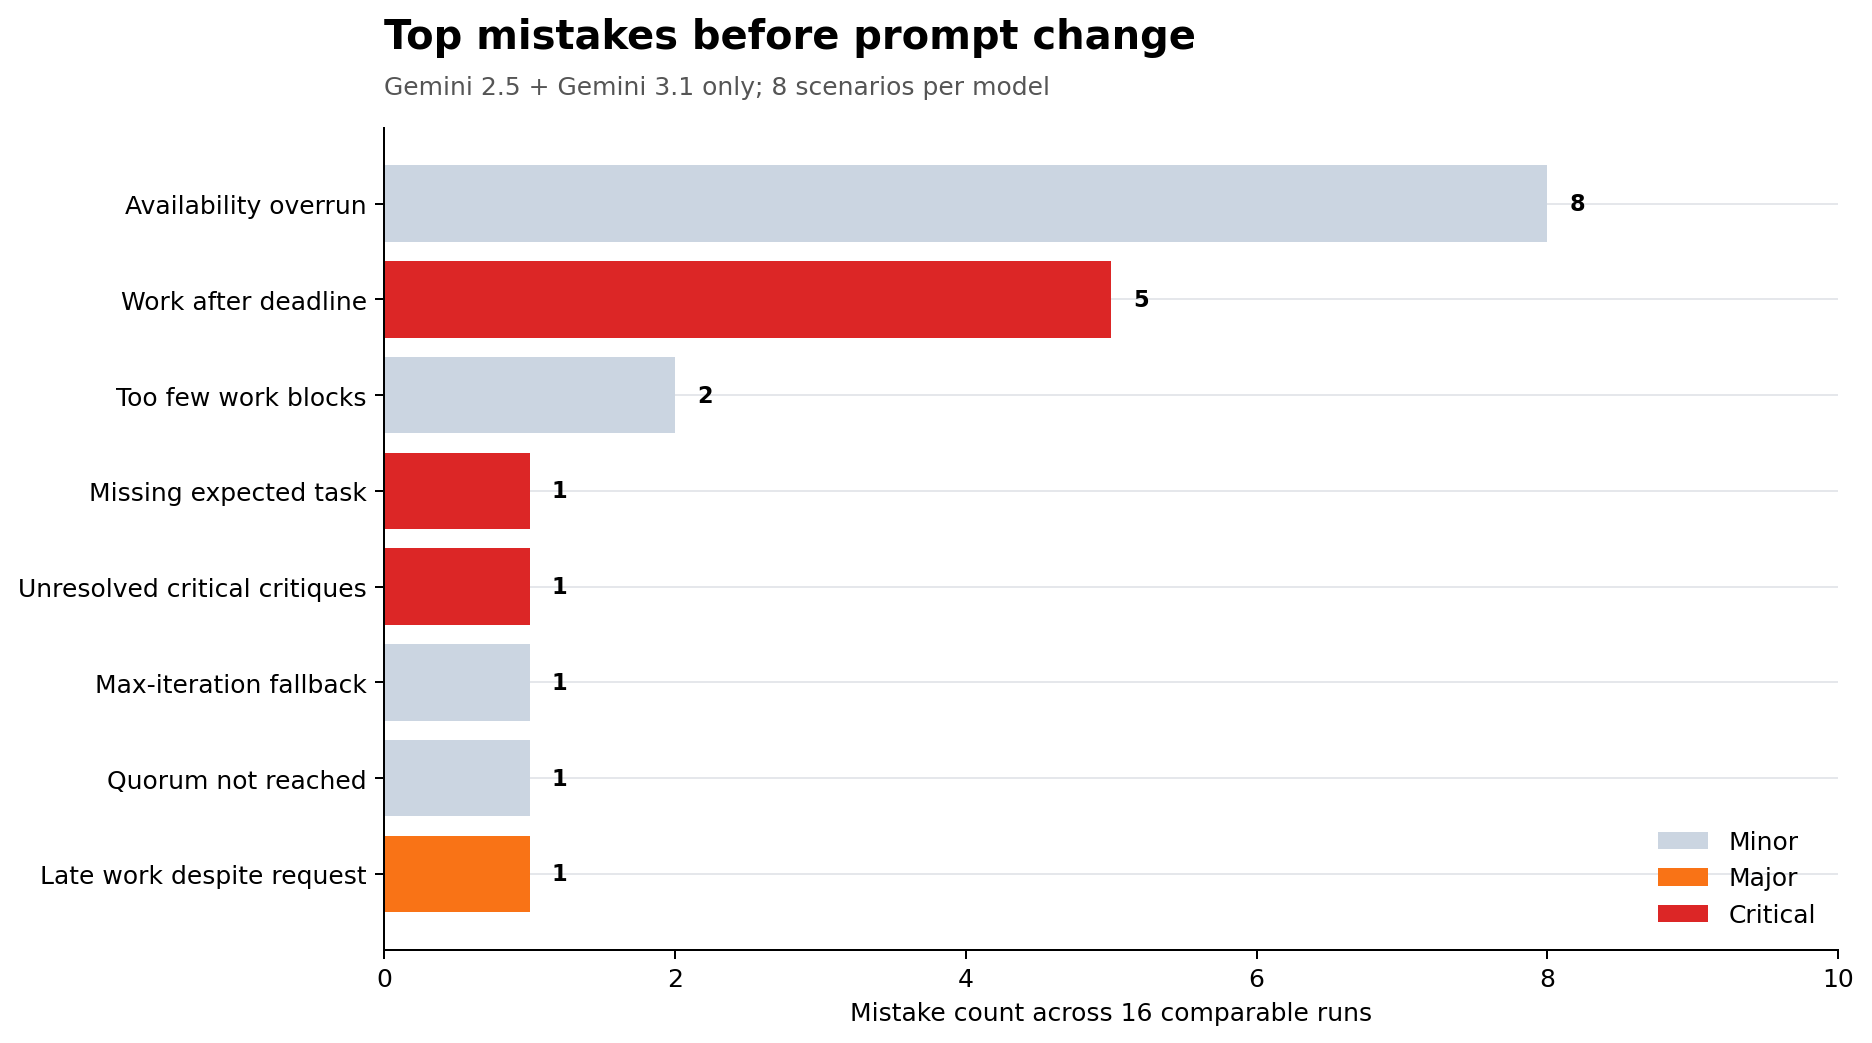
\includegraphics[width=\linewidth]{images/top_mistakes_before_prompt_change.png}
  \end{minipage}
  \hfill
  \begin{minipage}{0.49\textwidth}
    \centering
    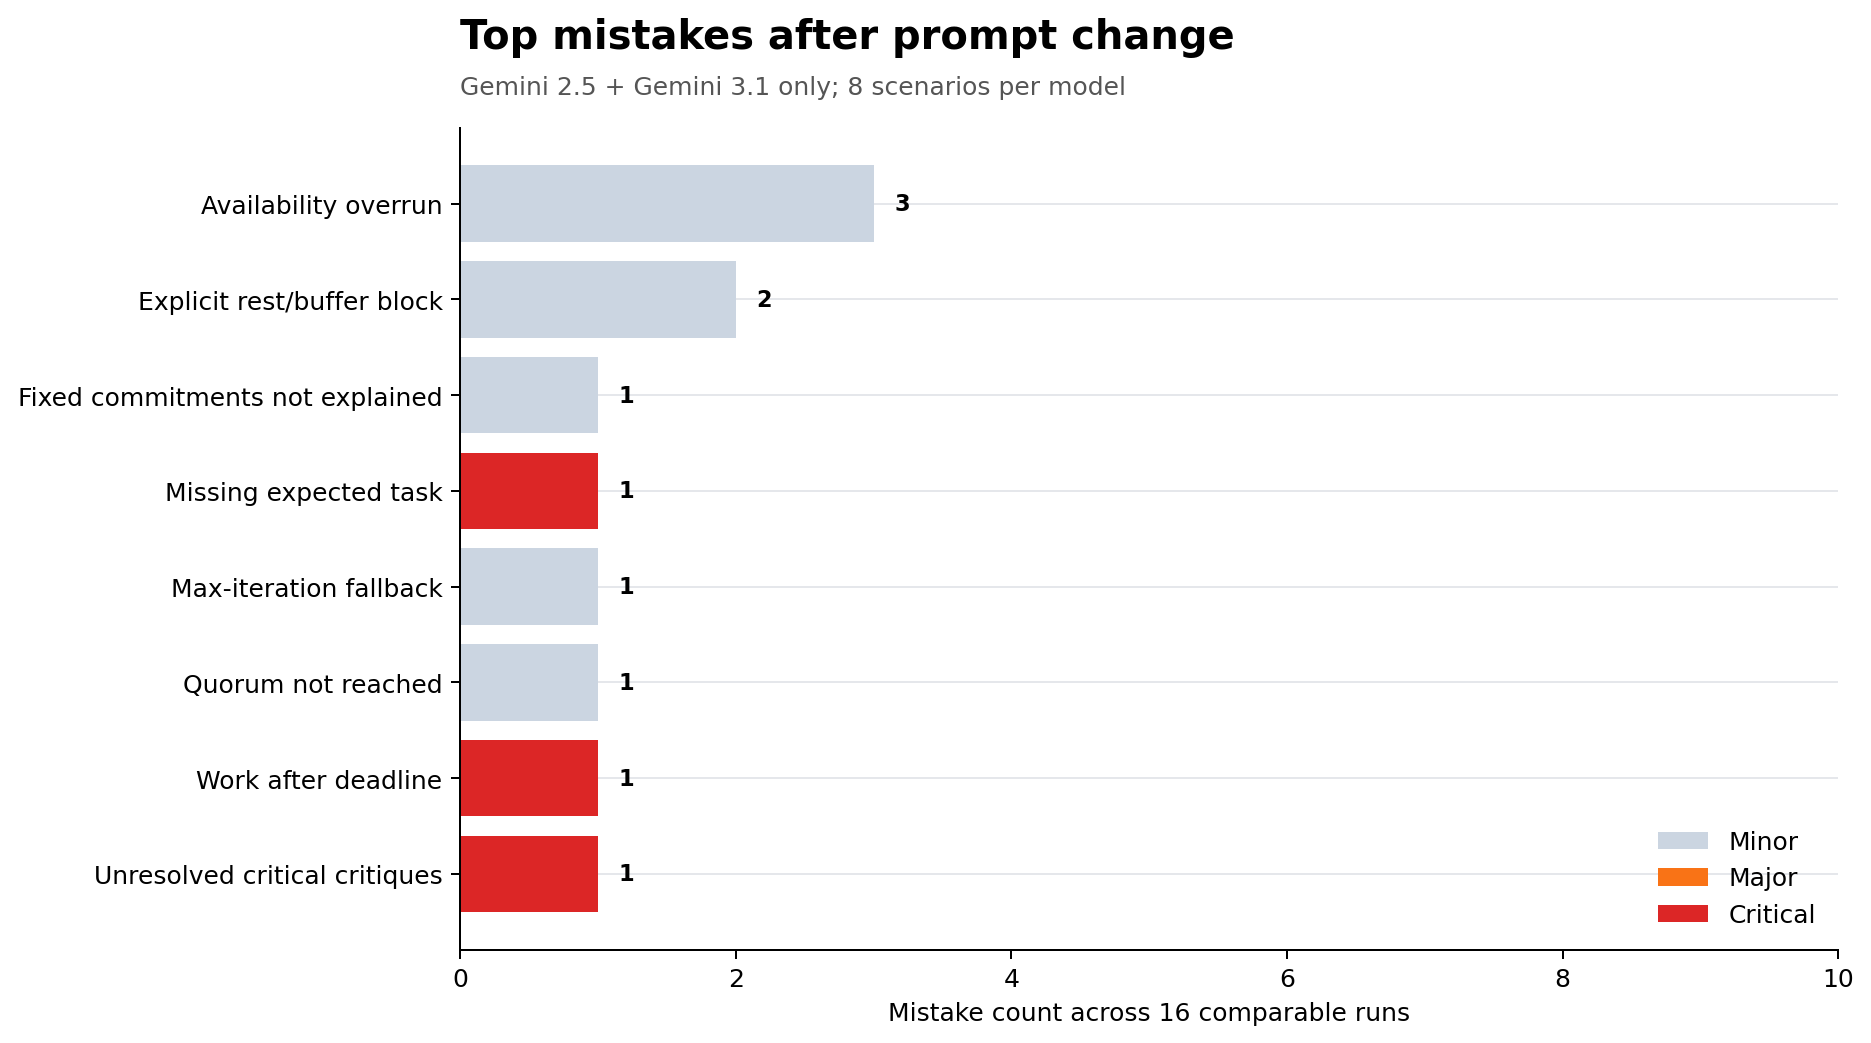
\includegraphics[width=\linewidth]{images/top_mistakes_after_prompt_change.png}
  \end{minipage}
  \caption{Top deterministic mistake labels before and after Deadline Agent prompt tuning. The comparison uses Gemini 2.5 and Gemini 3.1 over the same eight scenarios.}
  \label{fig:mistakes}
\end{figure*}

\section{Threats to Validity}
Two checks are necessary before making stronger scientific claims. First, our qualitative judge score uses one fixed evaluator model. This avoids the obvious error of each planner model grading its own output, but it does not prove that the evaluator is unbiased. The correct next experiment is to freeze the generated calendars and re-score them with multiple evaluator models, then report agreement, disagreement, and rank stability.

Second, the final comparison used a maximum of three iterations. The benchmark runner can vary this parameter, and we record the number of iterations actually used, but the final reported matrix does not yet contain a controlled one-versus-two-versus-three iteration ablation. That ablation should keep model, quorum, scenarios, and evaluator constant while varying only the maximum revision depth. It would show whether extra critique rounds reliably improve quality or mainly add cost and latency.

These gaps limit the strength of the evaluation claim. The supported claim is that the multi-agent loop is executable, auditable, and measurably improved by deterministic mistake labels. The broader claim that a specific evaluator, model, or iteration setting is generally optimal requires the two additional benchmark dimensions above.

\section{Conclusion}
Timebox demonstrates a practical multi-agent planning loop for student scheduling. The system produces calendars, exposes specialist critiques, and exports usable artifacts. More importantly, the evaluation loop turns subjective schedule generation into an auditable process: deterministic labels identify failure modes, prompt changes can be measured, and model choices can be compared by value rather than appearance alone. Future work should add multi-evaluator judging, iteration ablations, and larger scenario sets before making stronger model-selection claims.

\end{document}
